\chapter{Abstract}\label{cap:intro}

\begin{figure}[tbp]
\begin{center}
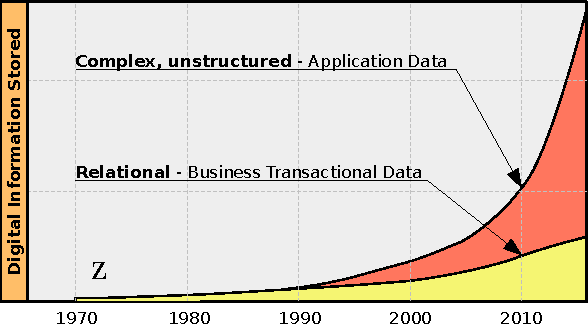
\includegraphics[width=0.99\textwidth]{imagenes/001.pdf}
 \caption{Demand in exponential growth. Source: \emph{Cloudera Inc.}}
\label{fig:datagraph}
\end{center}
\end{figure}

\noindent Over the last years there has been a continuous increase in the quantity of information generated with the Internet as the main driver. Furthermore, this information has reshaped from structured --- and thus, susceptible to being expressed following a relational schema --- to heterogeneous, which has kick-started the necessity to alter the way it is stored and transformed. As the figure \ref{fig:datagraph} shows, those that were the undisputed back-end queens --- relational database systems mostly --- are seeing how their role is fading away due to their incapability to efficiently save unrelated heterogeneity.

As another related dimension, in the year 2000 many .com companies started upgrading their data centers to accommodate the inexorable demand peak that was going to follow. But it never came; and the bubble burst. What happened then was general underutilization --- only \texttt{10\%} of Amazon's global computational resources were in use --- that pushed the search for alternative means to export the surplus as a product. Amazon's own initiative unfolded in 2006 with the \emph{AWS} (\emph{Amazon Web Services}) appearance. AWS, among others, implements a public API for flexible on-demand infrastructure provisioning.

Since then, similar projects have proliferated generalizing how private clusters' unused computational capacity is to be serviced, trying to stay API-compatible with the AWS to facilitate interoperability and thus avoid client's swapping to more flexible providers.

Meanwhile, Google was also in the search for new mechanisms to exploit, with high performance and securely, their own private infrastructure to evolve the capability of their services. MapReduce, as a way to massively execute thousands transformations on input data, became a reality to thrust the generation of Google's humongous inverted index of the Internet \cite{googlemapreduce}. Forthcoming contributions from Nutch's developers --- by that time an Internet search engine prototype --- to the MapReduce paradigm at \emph{Yahoo!}, would traduce into the appearance of today's \emph{de facto} standard in the field: Hadoop. Nowadays Hadoop is used in a myriad of backgrounds, ranging from travel booking sites to storing and servicing mobile data, ecommerce, image processing applications or searching for new forms of energy.

So, by stacking a MapReduce implementation atop elastic infrastructure an optimal exploitation of computational resources would be attainable, rapidly expanding or shrinking them on-demand, while simultaneously reducing the overall energy consumption required to accomplish processings (Figure \ref{fig:energysavings}).

\begin{figure}[tbp]
\begin{center}
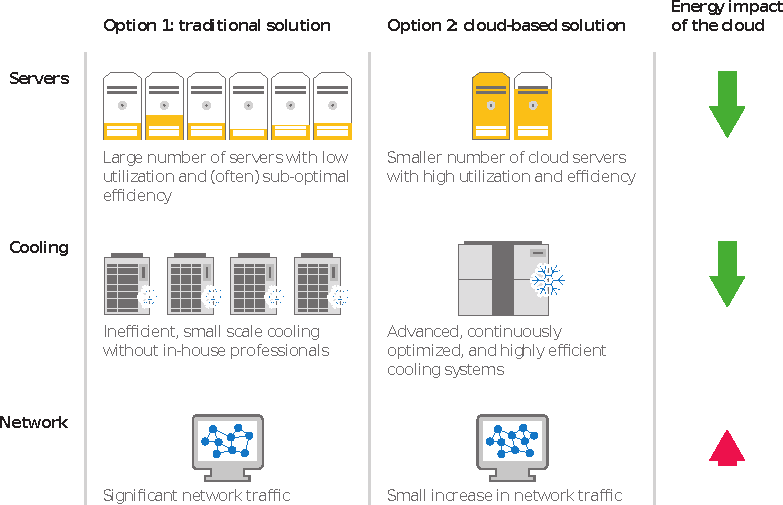
\includegraphics[width=0.99\textwidth]{imagenes/002.pdf}
 \caption{Motivaci\'on energ\'etica. Fuente: \cite{googleapps}}
\label{fig:energysavings}
\end{center}
\end{figure}



\section{Goals}\label{sec:objetivos}

\noindent El objetivo principal de este proyecto es estudiar la posibilidad de desarrollar una soluci\'on que permita dirigir el funcionamiento de un cloud para ejecutar algoritmia codificada siguiendo el paradigma MapReduce, reduciendo al m\'aximo la necesidad de conocimiento de la estructura del cloud concreto utilizado y de los par\'ametros de configuraci\'on de MapReduce.\newline

Para lograrlo se har\'a un an\'alisis pormenorizado de las variadas soluciones de creaci\'on de clouds. Se evaluar\'an sus capacidades y se configurar\'a un entorno de prueba utilizando virtualizaci\'on, que permita extraer conclusiones dirigidas a la elecci\'on de un \emph{framework} en concreto. Una vez completada la primera selecci\'on, se pasar\'a a la evaluaci\'on de los frameworks que soporten las caracter\'isticas del paradigma de programaci\'on MapReduce.\newline

Asimismo, se desarrollar\'a un mecanismo para el env\'io de peticiones de ejecuci\'on de trabajos MapReduce, centr\'andonos en la simplicidad y la universalidad de acceso de la interfaz con el cloud y MapReduce. Sin embargo, la sencillez no ha de representar un obst\'aculo para la explotaci\'on y la obtenci\'on de resultados. Del mismo modo, tanto la seguridad como la privacidad en las comunicaciones y el almacenamiento habr\'an de ser convenientemente definidas; no olvidemos que se trata la construcci\'on de un modelo reducido, a escala, de una soluci\'on que pueda ser implantable en una infraestructura infinitamente m\'as capaz.


\section{Organizaci\'on de la memoria}\label{sec:organizacion}
\noindent El contenido del presente documento se distribuye como se expone a continuaci\'on. Este primer cap\'itulo introduce la l\'inea general de desarrollo del proyecto. El cap\'itulo \ref{cap:estadodelarte} acerca al lector conceptos fundamentales de la \emph{computaci\'on cloud} ---como su arquitectura o la virtualizaci\'on--- y del paradigma MapReduce. El cap\'itulo \ref{cap:evaliaas} describe una evaluaci\'on pr\'actica de cuatro sistemas de manejo de clouds \emph{IaaS}. El cap\'itulo \ref{cap:openstack} explora la estructura modular y el funcionamiento particular de OpenStack Folsom. De forma an\'aloga, el cap\'itulo \ref{cap:hadoop} desvela las peculiarias de Hadoop como framework MapReduce. \newline

Los cap\'itulos subsiguientes se centran en detallar el proyecto desde distintos puntos de vista. El cap\'itulo \ref{cap:solucion} contiene las decisiones de dise\~no y los diagramas UML. El cap\'itulo \ref{cap:rendimiento} recoge los an\'alisis de rendimiento de la soluci\'on en un entorno real de pruebas. El cap\'itulo \ref{cap:conclusiones} analiza trabajos de investigaci\'on experimental relacionados con el proyecto, destacando comparativamente sus caracter\'isticas.  Finalmente, se resumen las principales aportaciones del proyecto y se proponen futuras mejoras a su implementaci\'on. \newline

Adicionalmente se han incluido dos anexos. El ap\'endice \ref{cap:guiainstalacion} recoge una gu\'ia r\'apida para la puesta en funcionamiento de una instalaci\'on del proyecto en un nodo. El ap\'endice \ref{cap:glosario} recoge las explicaciones de ciertos t\'erminos y tecnolog\'ias repartidas por todo el texto.
